\documentclass[a4paper, 12pt]{report}
\usepackage{tbagrelstandard}
\usepackage{charter}
\usepackage[skip=1.25\baselineskip]{parskip}

\title{
    Projet TOP 2018 \\%
    Groupe \sc{a2}%
}
\author{
    Axel \sc{Thouvenin}
    \and
    Florian \sc{Vogt}
    \and
    Pierre \sc{Bouillon}
    \and
    Thomas \sc{Bagrel}
}
\date{Novembre 2018 - Janvier 2019}

\newcommand{\tech}[1]{\sf{#1}}
\renewcommand{\tn}{\tech{TELECOM Nancy}}
\newcommand{\ext}[1]{\sc{#1}}
\newcommand{\gl}{\tech{GitLab}}
\newcommand{\en}[1]{\it{#1}}

\begin{document}

\maketitle

\tableofcontents{}

%================================================================================================================

% Mon estimation du temps (Thomas)
% - 30h dév Scala, 10h NodeJS + déploiement
% - 4h rapport
% - 4h Gestion de projet

% Florian
% - 15h dév Scala
% - 10h gdp/documents annexes
% - 5h rapport

% Axel
% - 10h dév Scala
% - 3h gdp
% - 5h rapport
% - 12h test

% Pierre
% - 20h dev Scala
% -  4h gdp (comptes rendus, production de docs/wikis, boards, etc.)
% - 10h tests
% -  4h intégration (gestion GitLab - essai de mise en place de CI)
% -  2h rapport

\part*{Introduction}\label{part:intro}
\addcontentsline{toc}{part}{\nameref{part:intro}}

Ce document a pour but de décrire l'évolution du projet que nous avons mené ces 3 derniers mois. Ce document contient cinq parties :
\begin{itemize}
    \item la première comporte une présentation générale du sujet, de l'interprétation que nous en avons faite, ainsi qu'un état de l'art analysant les technologies existantes traitant du même thème ;
    \item la deuxième décrit l'aspect technique de notre code, en particulier sa structure ainsi que les différentes technologies utilisées ;
    \item la troisième partie de ce rapport explore les techniques de test mises en place afin d'assurer le fonctionnement de notre code ;
    \item la quatrième partie vise à présenter la gestion de projet mise en place, son organisation concrète, les méthodes de travail que nous avons privilégiées (réunions, mesure de l'avancement\ldots{}) ainsi que les moyens de communication utilisés ;
    \item enfin, la cinquième et dernière partie a pour but de conclure sur le travail réalisé ainsi que d'exposer les perspectives d'évolution de notre projet.
\end{itemize}

Commençons tout de suite avec la présentation du sujet.

% Remerciements, et aussi on doit mettre les logos de nos entreprises respectives sur le rapport et la présentation (normalement)
% Docapost Applicam, Sopra Steria, Tracip et Euro Information

%================================================================================================================

\part{Le sujet}

\chapter{Exploration du sujet}

\section{Cadre général}

Ce projet a pris place pendant notre première année de formation Ingénieur apprenti à \tn{}. C'est l'école qui a fixé le sujet, que nous devions réaliser à la fois sur la période "école" mais également en partie en dehors, entre novembre 2018 et janvier 2019.

\section{Fichiers sources}

Le sujet se base essentiellement sur un fichier \ext{csv} (\en{Comma Separated Value}) fourni par le site \href{https://openflights.org/data.html}{\tt{openflights.org}}, qui recueille les données d'identités et de localisation d'un grand nombre d'aéroports à travers le monde : \href{https://raw.githubusercontent.com/jpatokal/openflights/master/data/airports.dat}{\tt{airport.dat}}

\section{Contenu du sujet et interprétation}

\subsection{Manipulations des données et statistiques}

Il nous était proposé de manipuler ce fichier afin d'en extraire plusieurs informations significatives, et en particulier, de calculer les distances séparant les différents aéroports. Ainsi, plusieurs questions du sujet nous proposaient de calculer la distance minimale, maximale, moyenne ainsi que l'écart-type des distances entre les différents aéroports.

Un autre axe du sujet, qui s'est révélé être déterminant pour notre choix de structure de code, était la possibilité de filtrer les aéroports suivant plusieurs critères : leur distance à un point quelconque, l'hémisphère ou encore le pays dans lequel il sont situés\ldots{}\\
En outre, il devait également être possible de calculer les statistiques évoquées ci-dessus sur un groupe d'aéroport restreint (filtré).

\subsection{Projection et affichage}

Les questions finales du sujet nous proposaient de projeter les aéroports sur une carte. Si ce volet ne laissait que peu de place à l'interprétation, le choix et l'étude des projections demandèrent tout de même un travail important.

Enfin, en dehors de ces questions explicitement présentes dans le sujet, nous avons été amenés à réfléchir méthodiquement aux structures de données et de code à utiliser afin de produire un code concis, clair, sans répétitions, et surtout modulable.

%================================================================================================================

\chapter{Etat de l'art}

Force est de constater que ce que nous avons réalisé est loin d'être novateur\ldots{} Par exemple, le site \href{https://openflights.org}{\tt{openflights.org}} duquel nous avons extrait nos données propose dès sa page d'accueil une carte dynamique des aéroports et des vols, bien au-dessus de ce que nous vous proposons ici.

Nous allons tout de même explorer les technologies les plus connues et utilisées dans les domaines que nous avons explorés.

\section{Données d'aéroports} Ici, \href{https://openflights.org}{\tt{openflights.org}} semble être le gagnant incontesté. En ce qui concerne les données sur les vols en direct (non couvert ici dans le sujet), on notera que \tech{Google} propose également un service de visualisation d'un vol dès que l'on tape un numéro de vol dans sa barre de recherche.

\section{Cartes et affichage}
\subsection{Données géographiques}
Concernant les données géographiques, deux géants s'affrontent : \tech{Google} avec \href{https://www.google.fr/maps}{\tech{Maps}}, et \href{https://www.openstreetmap.org}{\tech{OpenStreetMap}}, offrant des données totalement libres de droits, avec une communauté active et en pleine expansion.
\subsection{Affichage}
Concernant l'affichage (dynamique) de ces données géographiques, \tech{Google} joue ici un double rôle puisque \href{https://www.google.fr/maps}{\tech{Maps}} permet directement une visualisation dynamique de n'importe quel endroit du globe (mais encore une fois, avec une technologie propriétaire et fermée). Côté libre, cette mission est le plus souvent confiée à \href{https://leafletjs.com/}{\tech{Leaflet}} (utilisée sur le site de \href{https://www.openstreetmap.org}{\tech{OpenStreetMap}}), ou à \href{https://d3js.org/}{\tech{d3}} (que nous avons utilisé pour nos fonds de carte), deux librairies \tech{JavaScript} très populaires.

\section{Statistiques sur les aéroports}

Le calcul de statistiques de distance sur un groupe spécifique d'aéroports semble être une problématique trop précise pour trouver un service clé en main sur Internet. En effet, si une rapide recherche \sf{Google} nous permet de trouver une quantité incroyable de statistiques sur les aéroports pouvant intéresser les personnes prenant l'avion, nous n'avons pas pu trouver en ligne l'équivalent de ce que nous implémentons ici pour le projet (c'est-à-dire, sur les distances entre aéroports).

\section{Projections}

Nous avons brièvement étudié les projections existantes pour réaliser ce projet. Nous nous sommes surtout concentrés sur la projection équirectangulaire, comme demandé dans le sujet.

Seulement, il ne semblait pas exister sur Internet de définition précise de projection équirectangulaire centrée sur un point du globe. Nous avons donc décidé d'implémenter deux sous-types de projections équirectangulaires

\subsection{\tt{EquiRectangularLat0Projector}}

Cette projection centre horizontalement (en longitude) le point choisi, mais n'affecte pas les latitudes. Le planisphère est donc "enroulé sur lui-même" horizontalement par rapport à la projection usuelle centrée sur l'Europe. Les parallèles et les méridiens sont parallèles sur la carte obtenue. 

\subsection{\tt{EquiRectangularProjector}}

Cette projection centre horizontalement (en longitude) mais également verticalement (en latitude) le point choisi. Tout se passe comme si on faisait d'abord tourner le globe pour centrer le point choisi en longitude, puis qu'on faisait tourner le globe pour centrer le point choisi en latitude. Le point choisi se retrouve donc véritablement au centre de la carte finale, mais les pays sont "déformées" par rapport à la représentation usuelle centrée sur l'Europe (sauf dans le cas où la latitude du centre est $0$), et les parallèles et méridiens ne sont plus parallèles sur la carte obtenue.

\subsection{Autres projections}

Nous n'avons pas eu le temps d'implémenter d'autres types de projection, et donc nous n'avons pas regardé dans le détail les formules de projection associées. Seulement, notre code a été pensé dans le but de pouvoir implémenter \en{a posteriori} d'autres types de projections, y compris comme Mercator, où tous les points du globe n'apparaissent pas forcément sur la carte finale (avec notamment la classe abstraite \tt{ProjectedPoint}, se déclinant en \tt{OutOfMap} ou \\\tt{OnMap(x: Double, y: Double)}).

%================================================================================================================

% Montrer que le code est bon
\part{Développement}

    \chapter{Structure du projet} % diagramme, structure objet, pq on a choisis de faire de l'objet et aps autre chose
    
    \section{Introduction}

    Nous avons choisi, dès le début du projet, d'utiliser au maximum la puissance du langage imposé, \tech{Scala}, en alliant programmation fonctionnelle (pour la concision, la clarté, et la justesse du code) avec une structure objet, au travers des 
    \en{package}s, \en{module}s, \en{class}es, \en{trait}s et \en{object}s qu'offre ce langage.
    
    Ainsi, dès le premier commit (\href{https://gitlab.telecomnancy.univ-lorraine.fr/Projets_TOP/projet_top_a2/commit/6abc63fde8f6599fc6254ce4cfd0a93104ed4182}{\tt{commit/6abc63fde8f6599fc6254ce4cfd0a93104ed4182}}), la structure principale qu'allait revêtir notre code était déjà établie, permettant un repérage clair dans les tâches à réaliser ainsi qu'une compréhension facilitée de l'organisation et de l'utilisation de notre code.
    
    \section{Packages et classes}
    
    Héritant du \tech{Java}, l'organisation du code en \en{package}s de \tech{Scala} fut facile à prendre en main pour la plupart des membres du groupe. En revanche, la diversité des structures proposées par \tech{Scala} (\en{abstract class}, \en{class}, \en{trait}, \en{object}\ldots{}), souvent traduites indifféremment par des simples \en{class}es dans les langages objets courants, demanda plus d'efforts. Il fut décidé de les distinguer ainsi :
    \begin{itemize}
        \item \en{abstract class} : pour une classe "mère" décrivant un comportement générique, qui est ensuite spécialisé par les classes filles concrètes qui en héritent (exemple : \tt{AirportFilter}) ;
        \item \en{trait} :
            \begin{itemize}
                \item soit pour représenter une idée abstraite, une catégorie d'idées (\tt{enum}, exemple : \tt{HemisphereChoice}) ;
                \item soit pour représenter une "facette", un fragment de comportement que peut posséder un objet (exemple : \tt{HasCoordinate}, pour tous les objets possédant une localisation sur le globe au format longitude, latitude) ;
            \end{itemize}
        \item \en{object} :
            \begin{itemize}
                \item soit pour représenter une idée appartenant à une catégorie (membre d'une \tt{enum}, exemple : \tt{Northern} ou \tt{Southern}) ;
                \item soit pour regrouper les champs et méthodes statiques d'une classe (puisque contrairement au \tech{Java}, \tech{Scala} ne permet pas de placer de méthodes statiques dans ses classes) -- dans ce cas l'objet est appelé \en{companion object} ;
                \item soit, enfin, pour représenter tous les objets \en{singleton}s, c'est-à-dire le résultat de classes n'admettant qu'une seule instance (et donc instanciation) ;
            \end{itemize}
        \item \en{class} : pour toutes les classes restantes (et concrètes).
    \end{itemize}
    
    \section{Spécifique à \tech{Scala}}
    
    \subsection{Les \en{case class}es}
    
    On notera que les \en{case class} ont beaucoup été utilisées dans le code. En effet, ces dernières permettent un \en{pattern matching} facilité, et sont plutôt adaptées à représenter des structures de données immuables. Enfin, certaines de nos classes ne sont pas \en{case}, car les données passées en paramètres à leur constructeur nécessitent des petites modifications avant de devenir des attributs publics. Cependant, dans ce cas, nous avons implémenté les méthodes \tt{apply} et \tt{unapply} dans le \en{companion object} de la classe concernée, afin de bénéficier du \en{pattern matching} exactement comme pour une \en{case class} (voir diagramme de classe).
    
    \subsection{Les \en{lazy val}s}
    
    Nous avons changé une partie des méthodes de la classe \tt{AirportDistanceMap} par des \en{lazy val}. Ces dernières permettent d'allier le calcul sur demande des méthodes avec la persistance du résultat offert par une \en{val}. Pour résumer le fonctionnement des \en{lazy val}s, ces dernières n'évaluent le calcul que lors de l'appel, et le stockent ensuite comme une \en{val}. Ainsi, le calcul de la distance moyenne n'est effectué qu'au plus une fois par instance de la classe \tt{AirportDistanceMap}, et ce malgré son utilisation dans l'implémentation de la méthode du calcul de l'écart-type (\tt{stdDev}).

%================================================================================================================ 

    \chapter{Normalisation du code} % style / nomenclatures / appuyer sur le fait que ça soit très modulable et facilement maintenable / etc..
    
    \section{Introduction}
    
    La robustesse du code de notre projet est principalement apportée par sa structuration et l'utilisation des atouts de \tech{Scala}. Toutefois, nous avions tous conscience qu'un projet informatique est amené à être modulé et amélioré avec le temps (détection de bugs, ajout de fonctionnalités, etc.). Il nous a donc semblé crucial de pousser la rigueur avec laquelle développer jusque dans son style.
    
    \section{Style (pour le code)}
    
    \subsection{Choix du style}
    
    Ne pouvant perdre trop de temps à définir une nomenclature pour la totalité du langage, nous nous sommes largement appuyés sur une des normes en vigueur, à savoir celle de \href{https://docs.scala-lang.org/style/}{\tech{Scala}}.
    Nous disposions alors d'un wiki déjà fourni et avec quelques guides ; notamment pour l'utilisation de \tech{git} à ce moment. Notre choix a donc été d'ajouter une partie à la fin des tutoriels sur \tech{git} dans le wiki concernant certaines bonnes pratiques à prendre pour le code du projet. Elles sont disponibles \href{https://gitlab.telecomnancy.univ-lorraine.fr/Projets\_TOP/projet\_top\_a2/wikis/Helper\#bonnes-pratiques-de-d\%C3\%A9veloppement}{ici}.
    Nous y spécifions par exemple qu'il faut définir au mieux tout ce qui peut l'être, de lever les ambiguïtés qui peuvent apparaître et de produire du code aussi lisible qu'efficace.
    
    \subsection{Avantages apportés}
    
    Ce style de développement a permis une harmonisation entre le code de chacun et il était plus facile à la fois de s'inspirer de parties développées dans d'autres fichiers (car similaires et donc plus claires et explicites) ; mais aussi de mieux comprendre le travail des autres, en ne perdant pas de temps sur la forme et en pouvant directement se focaliser sur le fond et les algorithmes développés. Pour s'assurer de l'homogénéité du projet et de son style, les différentes méthodes d'intégrations mises en place à travers \tech{GitLab} nous permettaient à tous de progresser et d'ajuster le code rendu à chaque étape.
    
    Ces efforts sur la rigueur de l'écriture du code ont été payants surtout lors du début et de la fin du projet. Au début pour la compréhension globale des fichiers, et à la fin lorsqu'il nous a fallu améliorer et altérer certaines parties. La modularité de notre travail nous a permis de gagner un temps considérable lorsque des modifications étaient nécessaires, permettant d'éviter l'introduction de bugs (car le code aurait été abscons), et permettant également d'éviter de déranger l'auteur du-dit code. Il en résulte un code propre, stable de par sa structure et fluide de par sa forme.
    
    \section{Complexité}
    
    La seule complexité notable de notre projet est la création de l'objet \tt{AirportDistanceMap}, puisque, lors de l'exécution de l'algorithme, il s'agit de calculer des données relatives aux aéroports entre eux. De fait, il nous fait itérer deux fois sur chaque élément du tableau. Il en résulte une complexité en n carré qui, bien que peu élégante, est malheureusement nécessaire pour cette partie.
%================================================================================================================

    \chapter{Technologies} % parsing CSV / etc.
    
    \section{Parsing du CSV}
    
    \subsection{Choix de la librairie}
    
    Afin de lire les fichiers d'aéroports et de pays (au format \ext{.csv}), nous avons choisi de faire appel à une librairie externe afin de respecter le principe \en{don't reinvent the wheel}, et surtout d'éviter d'introduire des bugs potentiels supplémentaires dans notre \en{codebase}.
    
    Nous avons choisi la librairie grâce à \href{https://github.com/lauris/awesome-scala}{\tech{awesome-scala}}, un \en{repo} \tech{GitHub} présentant les meilleures et plus populaires librairies en \tech{Scala} pour de nombreux usages.
    
    Notre choix s'est donc porté sur \href{https://github.com/tototoshi/scala-csv}{\tech{scala-csv}}, sous licence \href{http://www.apache.org/licenses/LICENSE-2.0}{Apache 2.0}.

    \subsection{Avantages apportés}
    
    L'utilisation d'une librairie nous a permis de bénéficier d'un \en{parsing} du CSV à la fois plus performant et plus complet que l'implémentation maison que nous aurions pu produire. Par exemple, nous n'avons pas eu besoin de gérer les cas où les champs CSV contiennent eux-mêmes une virgule (et nécessitent donc un échappement avec des guillemets), ce qui aurait été fastidieux et peu intéressant à faire à la main dans le cadre de ce projet.
    
    \section{Construction de la carte}
    
    Pour construire la carte, nous avons utilisé la librairie \href{https://docs.oracle.com/javase/7/docs/api/java/awt/package-summary.html}{\tech{java.awt}}, conseillée pour \tech{Scala}, et disposant au final de méthodes pratiques pour travailler sur une image (\ext{.png}).
    
    C'est notamment à partir des composants de \tech{java.awt} que nous avons développé nos classes \tt{Marker}, pour ajouter un marqueur sur le fond de carte fourni par le \tt{BackmapProvider}
    
    Au final, l'écosystème \tech{Java}/\tech{Scala} aura été très utile pour trouver facilement des librairies performantes et documentées pour nous aider dans la réalisation du projet

%================================================================================================================

\part{Réalisation des tests}
    \chapter{Méthodologie}
    
    \section{Tests unitaires ou non ?}
    
    Il existe de nombreuses façons de réaliser des tests unitaires, chacune étant plus ou moins rigoureuse et/ou fidèle au principe "unitaire" du test. Pour cette raison, il nous fallait avoir des tests cohérents à la fois dans ce qu'ils testent, mais aussi entre eux, que chaque test soit tout autant pertinent que les autres présents.
    
    Pour cela, nous avons choisi de structurer la réalisation de nos tests, qui se sont faits selon certains critères
    
    \section{Implémentation}
    
    Pour chaque bout de code, le test en lui-même doit respecter certaines règles. Ainsi, il ne faut pas qu'il appelle de composantes externes, pour respecter le caractère unitaire du test. Par exemple, une méthode testée d'un objet ne doit pas en appeler une autre dans le même test. 
    
    Pour éviter de tomber dans les travers du test, nous avons tout de même procédé à quelques limitations : les méthodes de \tech{Scala} ne doivent pas être testée (si \tech{Scala} propose une méthode, rien ne sert de vérifier qu'elle fonctionne dans notre propre méthode) et il est inutile de tester les frameworks utilisés (ils sont supposés stables et déjà testés). Une autre contrainte implicite a été respectée, à savoir ne pas surcharger de tests le projet. Ils sont en effet nécessaire pour contrôler son évolution, mais trop en avoir aurait eu l'effet inverse en enlevant toute flexibilité et en rigidifiant les possibilités offertes par le code. Nous nous sommes donc "limités" à des tests pertinents assurant que le fonctionnement des méthodes est correct.
    
    \section{Méthodologie AAA}
    
    Plus verbeusement \en{Arrange Act Assert}, cette méthodologie se décompose comme son nom l'indique en trois phases. Initialement, on crée les composantes à tester et les valeurs à leur associer (\en{Arrange}) ; on effectue ensuite l'action qui va être testée, en récupérant son retour s'il existe (\en{Act}) ; finalement, on vérifie le résultat en le comparant à un résultat attendu (\en{Assert}).
    
    De cette manière, chaque test est extrêmement lisible et concis : on sait ce qui est testé, comment, et quel retour est attendu.
    
    \chapter{Frameworks}
    
    \section{Choix du framework}
    Le choix du framework de test est extrêmement important et a nécessite une véritable réflexion. En effet, peu importe les efforts déployés dans la structuration, si les tests de part leur nature n'étaient pas construit autour de la même optique, nous allions alors avoir des dissonances et perdre en efficacité.
    
    Ainsi, différents frameworks ont été explorés et plus ou moins contestés.
    
    \section{FeatureSpec}
    
    FeatureSpec nous a semblé intéressant grâce à sa syntaxe, proche de celle du SQL avec un principe de mots clefs clairs et un détail de chaque scénario. Cependant ce choix a vite été abandonné car devant la redondance de certains tests et la différence entre la taille des tests (de quelques lignes à plusieurs blocs) il nous a semblé que nous allions très rapidement nous retrouver avec des tests, bien que bien structurés, totalement illisibles et difficilement maintenables.
    
    \section{WordSpec}
    
    WordSpec avait l'avantage de la concision et de rester verbeux même si réduit. On retrouvait ce principe de mots clefs pour garder un aspect très lisible et compréhensible, mais la succession de ces derniers impliquait une imbrication selon les cas pouvant devenir très importante trop rapidement.
    
    N'ayant pas encore idée de la structure de tous nos tests ou de leurs complexités dans leur rédaction, nous avons préféré explorer d'autres pistes.
    
    \section{FunSuite}
    
    FunSuite est très simple d'utilisation et très similaire à de nombreux autres frameworks de tests. Nous avons abandonné cette initiative au profit d'une solution, au risque d'être plus complexe, nous dotant d'outils plus puissants; voire une meilleure structuration dans la synthaxe de nos tests.
    
    \section{FlatSpec}
    
    FlatSpec a un aspect très fluide dans son écriture: les mots clefs et la "documentation" s'enchevêtre très bien et nous permette d'écrire des tests tant élégants, que maintenable, que lisibles et efficaces.
    
    
    % analyse des frameworks et choix de scalatest flatspec
    \chapter{Structuration des tests}
    
    Le rôle particulier des tests dans un projet tends à faire défaut à la qualité avec laquelle ils sont produits. On voit souvent des tests peu utiles, pertinents, voire parfois même, leur absence totale.
    
    C'est pour éviter ces travers courant que nous avons préféré dès le début maintenir la même rigueur et exigence pour les tests que pour le code.
    
    Afin de rester clair et explicites, nous avons choisi que pour chaque fichier de code, correspondra un fichier de tests. Cette structure quasi dupliquée des fichiers permet du premier coup d'oeil de saisir à quel fichier correspond quel test. Pour renforcer cette rigidité, nous avons associé un objet de test par méthode testée. Une méthode d'un fichier avait donc, pour tests, un fichier correspondant dans lequel se trouvait un objet Scala, testant les différents comportement de notre code.
    
    Pourtant, nos tests utilisant parfois des ressources communes, nous souhaitions continuer à préserver ce principe de \en{DRY} (Don't Repeat Yourself). C'est pourquoi la structuration des fichiers tests diffèrent en quelques points, dont celui de fichiers ressources utiles spécialement aux tests se trouvant dans le répertoire consacré à ces derniers.

%================================================================================================================

\part{Gestion de projet}

    \chapter{Choix de la méthodologie} % orga de notre SCRUM + répartition travail / tps de sprints
    Nous avons opté pour un processus agile en combinant les méthodes agiles SCRUM et Kanban (Sprint Backlog) tout en s'inspirant du cadre agile "eXtreme Programming" qui nous a permis de notamment renforcer plusieurs points importants.
    
    \section{Intégration des modifications}
    
    Les "branches" de \gl{} nous ont permises de séparer proprement les tâches à effectuer. En effet, lorsque nous voulions travailler sur un point précis, la première chose que nous faisions était de créer une branche pour celui-ci. Ensuite, nous réalisions la tâche (soit seul soit à plusieurs) puis lorsque l'équipe attribuée considérait que le développement était fini, elle le signalait aux autres membres du projet en créant une \en{Merge Request}, et ces derniers procédaient alors à des revues de code.
    
    \section{Revues de code}
    
    Représentées par les \en{Merge Requests} (MR) de \gl{}, à la fin du développement de la tâche par l'équipe désignée, celles-ci proposaient une fusion avec le projet principal où les autres membres du groupe devaient analyser les changements effectués par cette branche, puis les valider ou refuser en justifiant par le biais de commentaires la modification. Ce fonctionnement nous a permis de chacun voir ce que les autres avaient réalisé.
    
    \section{Cycles de développements rapides}
    
    Nos sprints ont tous duré deux semaines, ce qui nous a permis de bien développer les fonctionnalités cruciales du projet assez rapidement. En plus des stand-ups meetings, en milieu de sprint (chaque semaine), nous réalisions des réunions d'avancement, afin de mettre en avant les problèmes rencontrés et éventuellement les corriger afin d'éviter tout blocage éventuel.
    
    \chapter{Réunions et jalons}
    
    \section{Description des jalons}
    
    Au début du projet, nous nous sommes réunis afin de définir des catégories de jalons :
    \begin{itemize}
        \item \en{Open} : Élément non traité et qui ne le sera pas dans le sprint en cours ;
        \item \en{To implement} : Élément à implémenter dans le sprint en cours ;
        \item \en{Implementing} : Élément en cours d'implémentation ;
        \item \en{To Test} : [Dans le cas d'un algorithme] Élément développé nécessitant des tests unitaires ;
        \item \en{Testing} : Élément pour lequel les tests unitaires sont en cours de rédaction ;
        \item \en{To Review} : Élément à vérifier (développement et tests réalisés (dans le cas d'un algorithme), bien rédigés (dans le cas d'un document) \ldots{});
        \item \en{Reviewing} : Élément en cours de vérification;
        \item \en{Closed} : Élément terminé : implémenté, testé et/ou vérifié.
    \end{itemize}
    
    Ils étaient donc tous référencés parmi celles-ci sur l'\en{issue board} de \gl{} (qui nous a servi de \en{Sprint Backlog} / tableau Kanban).
    Celui-ci était mis à jour constamment et était utilisé lors de chaque réunion en tant qu'appuis aux discussions.
    
    \section{Réunions}
    
    Tous les lundis, nous réalisions une réunion de type "avancement", afin de faire le point sur les tâches qui avaient déjà été réalisées en mi-sprint ou pour clôturer le sprint en cours et ainsi commencer le suivant.
    
    Celles-ci nous servaient à communiquer sur les points importants qui nécessitaient une discussion plus longue (rapports sur l'avancée, prises de décisions \ldots{}), en plus des stand-ups meetings quotidiens qui servaient eux à traiter les petits problèmes (question(s) sur la partie d'un autre membre, demande de \en{code review} \ldots{}) .
    
    De plus, il nous arrivait de nous réunir physiquement afin de porter une réflexion commune sur un sujet plus important que le développement d'une fonction (principalement un changement de structure ou un ajout important, ex : les projections) et qui ne pouvait attendre une réunion planifiée.
    
%----------------------
    
    \chapter{Organisation du travail} % wbs, etc **REPARTITION ENTRE LES GENS DES TESTS + ISSUES + Orga en KANBAN (boards) **
    
    \section{Kanban}
    
    \subsection{\en{Issue board}}
    
    Puisque nous avons choisi d'adopter une approche agile, nous avons donc planifié nos tâches pendant nos réunions d'amorçage de sprint (catégorie \en{To implement}), puis nous les avons réparties entre nous par compétence et affinité, sur le tableau Kanban (\en{Sprint Backlog}) que propose \gl{} (qui est normalement le "tableau de problèmes" (\en{issue board}) pour les communautés de plus grande ampleur).
    
    \subsection{\'Evolution incrémentale}
    
    Afin d'assurer un suivi du tableau au fur et à mesure de l'avancement des tâches, celles-ci étaient déplacées dans la catégorie correspondante à leur statut actuel de façon incrémentale : lorsque le développement était fini, elle se devait d'être testée (dans la limite du possible) puis ensuite être revue pour affirmer que son intégration dans le code resterait une évolution (sans \en{continuous integration}).
    
    \subsection{Branches}
    
    Dès la première réunion, nous avons débattu afin d'adopter un mode de fonctionnement pour la mise en commun du travail en utilisant \gl{} : nous avons retenu un fonctionnement par branches, avec comme contrainte d'ajouter une fonctionnalité supplémentaire ou d'améliorer le projet en général, puis, lorsque celle-ci était fusionnée avec la branche mère (\tt{master}), la branche était automatiquement supprimée avec l'option disponible lors de la création des \en{Merge Requests}.
    
    \section{Aperçu des sprints réalisés}
    
    Voici un schéma récapitulatif de nos sprints :
    \begin{figure}[h]
        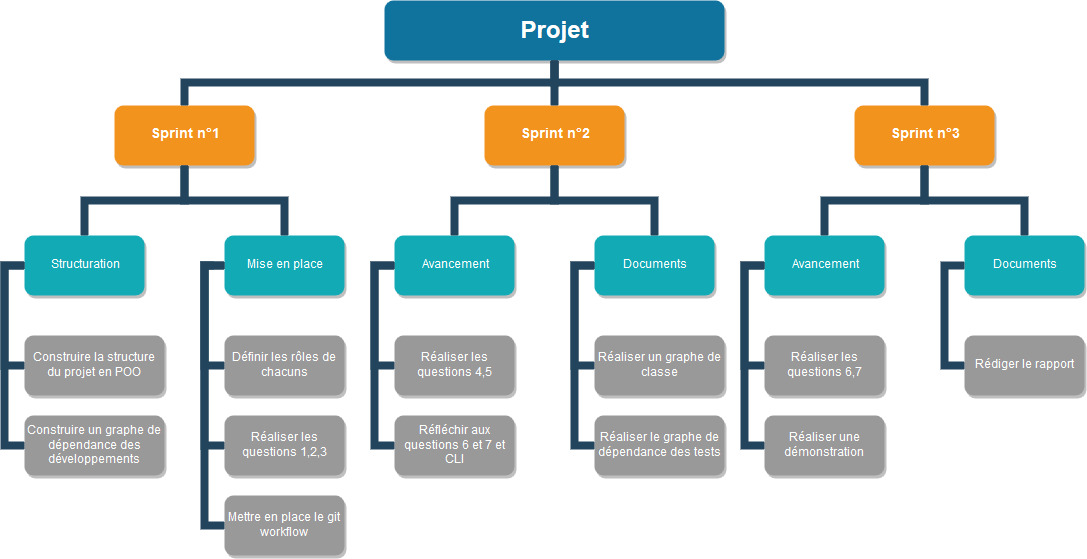
\includegraphics[width=\textwidth]{resources/WBS.jpg}
        \centering
            \caption{\label{1} Répartition des sprints}
    \end{figure}
    
    Toutefois, les tâches ne se limitaient pas au développement, il nous a fallu rédiger quelques documents annexes afin de mener à bien ce projet, tel qu'un diagramme de classe dans le but de se retrouver parmi nos objets et nos méthodes.
    
    \chapter{Difficultés rencontrées} % pair programming, homogeneité des niveaux de chacuns, delais
    
    \section{Niveaux des membres du groupe}
    
    La première difficulté qui s'est révélée au début du projet est le niveau non homogène des membres du groupe, nous avons donc choisi de résoudre ce problème lors de la répartition des tâches : les fonctions simples se sont donc plus réparties sur les personnes plus faibles de l'équipe tandis que les points plus complexes se sont vus réalisés à plusieurs (\en{pair programming}) afin que chaque membre du groupe puisse progresser dans ces domaines.
    
    % mise en place de la cli, le rapport, les finitions, le refactoring, short de boucler
    \section{Gestion du temps}
    
    Nous avons également eu des difficultés à maintenir un rythme constant, car certains points indispensables du projet nous ont pris plus de ressources que prévu, 

    De plus, le problème du temps s'est accru lorsque nous avons essayé d'implémenter des fonctionnalités qui se sont avérées difficiles à implémenter sans être primordiale, en particulier la CI/CD (\en{Continous Integration / Continuous Deployment}) sur \gl{}.
    
    \chapter{Communication interne} % Discord / GitLab / MR
    L'une des notions les plus importantes à la réalisation d'un projet est la communication. Nous avons choisi de ne pas négliger cela et avons mis en place plusieurs moyens de dialogue :
    
    \section{\tn{}}
    
    Notre moyen d'échange le plus utilisé a été l'enseigne même de l'école \tn{}. En plus de nos réunions régulières, nous utilisions notre temps libre afin de parler du projet et de nos différents problèmes rencontrés durant nos sprints.
    
    \section{\tech{Discord}}
    
    Nous avons beaucoup utilisé \tech{Discord}, un logiciel gratuit optimisé pour la communication rapide. Nous avons créé des salons textuels portant des noms spécifiques permettant de garder une certaine rigueur et d'optimiser notre partage d'informations. Grâce à cela nous étions capables contextualiser la demande très rapidement. Nous avons également mis en place des salons vocaux principalement consacrés au \en{pair programming}.
    
    \section{\gl{}}
    
    \gl{} nous a permis de suivre le projet dans son ensemble et de lire le code en son intégralité à travers les différentes \en{Merge Request}s. \gl{} nous a permis également de laisser une trace de la répartition des tâches dans le groupe. ;

%================================================================================================================
    
\part{Bilan et évolutions}
    
    \chapter{Bilan} % bilan du travail réalisé / comptabilisation de l'expérience / couverture de tests / CI 
    
    Arrivé à la date butoir du rendu de projet, nous avons un code fonctionnel, performant et testé. De plus, il couvre l'ensemble des problématiques du sujet, sans aucun comportement anormal ou défaut de fonctionnement.
    
    L'utilisation de GitLab et du \en{VCS} git s'est également très bien déroulée, avec un \en{git history} propre, cohérent, illustrant bien l'implication et les évolutions du projets tout au long de son développement.
    
    Pour finir, la réalisation ponctuelle mais efficace de réunions d'avancements et de stand-up meeting nous a maintenu sur la bonne voie en renforçant à la fois la cohésion mais aussi la visibilité globale du projet et de ses difficultés par tous les membres du groupe.
    
    Il en résulte un livrable fini, de qualité ainsi que des documents l'accompagnant fournis. A défaut peut-être d'une gestion du temps parfois un peu trop approximative, l'expérience tirée par les membres du groupe est à la hauteur de la qualité du projet ainsi réalisé.
    
    
    \chapter{Évolutions possibles} % perspectives d'avenir (i.e. lier en temps réel, ajouter une interface, ajouter un mode sattelite.. ajouter new prokection, cli devient api )
    Durant la réalisation du projet nous nous sommes rendu compte que certains points pouvaient être améliorés :
    \begin{itemize}
        \item Ne plus faire appel a un fichier sous forme csv pour le chargement des données, mais faire directement appel a une Api ce qui permet une mise à jour des données. Exemple, si un pays change de nombres d'aéroports cela changera aussi dans l'API.
        \item Avoir une vue satellite de notre carte pour une meilleure visualisation. Nous avions essayé mais la taille de l'image était trop importante.
        \item Approfondir encore plus loin les projections proposées par notre programme.
        \item Remplacer notre CLI par une API. Donc de ne plus avoir à passer par des commandes mais par une interface graphique routée par un serveur web.
    \end{itemize}

%================================================================================================================
    

\part*{Annexes}\label{part:annexes}
\addcontentsline{toc}{part}{\nameref{part:annexes}}

\chapter{Compte-rendus de réunions}
%%%%%%<inclure diagramme de classe>

%=============================================================
%=============================================================
%=============================================================

\section{Compte rendu de réunion \no{0}}
\subsection*{Membres présents:}

\begin{itemize}

\item
  Bagrel Thomas
\item
  Bouillon Pierre
\item
  Thouvenin Axel
\item
  Vogt Florian
\end{itemize}

\subsection*{\texorpdfstring{Sujet: \emph{Structuration et mise en place du projet}}}

\subsection*{Ordres du jour:}

\begin{itemize}

\item
  Critique et retour sur le WBS
\item
  Point sur le git workflow
\item
  Réflexion sur les tests et la structure du code
\end{itemize}

\subsection*{Général}

\subsubsection*{WBS}

\begin{itemize}

\item
  Raffinement de la répartition des tickets
\item
  Satisfaction globale du groupe: clair, efficace et synthétique
\end{itemize}

\subsubsection{Workflow}

\begin{itemize}

\item
  Utilisation du branching workflow (une fonctionnalité = une branche
  séparée)
\item
  Présence d'un wiki, le centraliser sur le GitLab
\item
  Quelques zones d'ombre sur l'utilisation du workflow ont été
  redétaillées
\item
  Mise en place de pair-programming pour accompagner les membres dans
  l'utilisation du workflow
\end{itemize}

\subsubsection{Tests et structure}

\begin{itemize}

\item
  Réflexion sur un framework de test pour effectuer des tests unitaires
\item
  Déconstruction des tests sous la forme AAA* évoquée
\item
  Difficulté pour rédiger les tests unitaires à cause de parties
  interdépendantes pas encore implémentée =\textgreater{} Construction
  d'un graphe de dépendances pour prioriser les implémentations
\item
  Workflow type à terme: implémentation -\textgreater{} documentation
  -\textgreater{} test -\textgreater{} review
\end{itemize}

\begin{itemize}

\item
  \href{https://www.c-sharpcorner.com/UploadFile/dacca2/fundamental-of-unit-testing-understand-aaa-in-unit-testing/}{AAA
  testing}
\end{itemize}

%=============================================================
%=============================================================
%=============================================================

\section{Compte rendu de réunion \no{1}}

\subsection*{Membres présents:}

\begin{itemize}

\item
  Bagrel Thomas
\item
  Bouillon Pierre
\item
  Thouvenin Axel
\item
  Vogt Florian
\end{itemize}

\subsection*{Sujet: \emph{Avancement}}

\subsection*{Ordres du jour:}

\begin{itemize}

\item
  Priorisation des tâches
\item
  Mise en commun de la progression de chacun
\end{itemize}

\subsection*{Général}

\subsubsection*{Priorisation des tâches}

\begin{itemize}

\item
  Graphe de dépendance des tests finis: organiser la rédaction des tests
  autour dudit graph
\item
  Implémenter les tests tels que la personne les ayant fait ne les codes
  pas mais review la PR les concernant
\item
  Au choix du développeur parmi le label \texttt{to\ test}
\end{itemize}

\subsubsection{Mise en commun de la progression de chacun}

\begin{itemize}
\item
  Bagrel Thomas

  \begin{itemize}
  
  \item
    Fin des issues à développer
  \item
    Début du testing dès l'ajout d'un template de test
  \item
    Implémentation de la distance entre les aéroports
  \end{itemize}
\item
  Bouillon Pierre

  \begin{itemize}
  
  \item
    Fin des tâches sur les Airports
  \item
    Modifier l'unité du \texttt{.csv} des \texttt{countries} et
    implémenter sa lecture
  \item
    Ajout de ressources dans le wiki
  \item
    Voir pour l'implémentation GitLab de l'intégration continue
  \end{itemize}
\item
  Thouvenin Axel

  \begin{itemize}
  
  \item
    Pair-programming
  \item
    Prise en main du projet, prise de conscience des issues
  \end{itemize}
\item
  Vogt Florian

  \begin{itemize}
  
  \item
    Issues avancées mais pas encore push (sera fait dans la soirée)
  \item
    Graphe de classes à faire
  \item
    Diagramme de classes à faire
  \end{itemize}
\end{itemize}

%=============================================================
%=============================================================
%=============================================================

\section{Compte rendu de réunion \no{2}}

\subsection*{Membres présents:}

\begin{itemize}

\item
  Bagrel Thomas
\item
  Bouillon Pierre
\item
  Thouvenin Axel
\item
  Vogt Florian
\end{itemize}

\subsection*{Sujet: Revue du sprint \no{1}}

\subsubsection*{Points positifs}

\begin{itemize}

\item
  Gitlow, système de board et de marge requests très fluides et
  appréciés;
\item
  Code et architecture propres, agréable à review et explicite;
\item
  Diagramme UML qui permet de bien appréhender le projet dans son
  ensemble.
\end{itemize}

\subsubsection*{Points négatifs}

\begin{itemize}

\item
  Tracking des issues à tester peut-être pas assez rigoureux;
\item
  Attention à garder une avance vis-à-vis de la deadline.
\end{itemize}

\subsubsection{Améliorations suggérées}

\begin{itemize}

\item
  Possibilité de générer un manuel technique du logiciel grace à la
  ScalaDoc;
\item
  Prévenir dans les channels de communication intra-groupe pour prévenir
  des MR.
\end{itemize}

\subsubsection{Tâches reportées}

\begin{itemize}

\item
  Continuer à tester les différentes classes et atteindre une plus
  grande couverture de code testé.
\end{itemize}

\subsubsection{Autre}

\begin{itemize}

\item
  Evocation d'une évolution du workflow en branches avec différents
  niveaux de maturité (non suivie à cause de l'impact en terme de temps
  et de complexité que ça impliquerai)
\end{itemize}

%=============================================


\section{Compte rendu de réunion \no{3}}

\subsection*{Membres présents:}

\begin{itemize}

\item
  Bagrel Thomas
\item
  Bouillon Pierre
\item
  Thouvenin Axel
\item
  Vogt Florian
\end{itemize}

\subsection*{Sujet: Amorçage du sprint \no{2}}

\subsection*{Ordre du jour:}

\begin{itemize}

\item
  Planification des tâches
\end{itemize}

\subsection*{Général}

\subsubsection*{Planification}

\begin{itemize}

\item
  Répartition des différentes tâches dans le board;
\item
  Implémentation des questions 6/ et 7/;
\item
  Continuation des tests;
\item
  Evocation d'une interface (?);
\item
  Tâches annexes:

  \begin{itemize}
  
  \item
    Tests intégration en corrélation avec le Readme.md;
  \item
    Etudier la mise en place de la CI;
  \item
    Implémenter une méthode qui appellerait une API pour les
    \texttt{Countries};
  \item
    Nourrir le wiki;
  \item
    Etudier l'utilisation de lazyvals;
  \item
    Refactoring de certains noms d'attributs.
  \end{itemize}
\end{itemize}

%================================

\section{Compte rendu de réunion \no{4}}

\subsection*{Membres présents:}

\begin{itemize}

\item
  Bagrel Thomas
\item
  Bouillon Pierre
\item
  Thouvenin Axel
\item
  Vogt Florian
\end{itemize}

\subsection*{\texorpdfstring{Sujet: \emph{Avancement}}}

\subsection*{Ordres du jour:}

\begin{itemize}

\item
  Remarques et ressentis sur l'avancement du sprint
\end{itemize}

\subsection*{Général}

\subsubsection*{Remarques négatives}

\begin{itemize}

\item
  De gros ralentissement liés à un problème coté GitLab qui tuais la
  fluidité du workflow à cause de l'impossibilité de merge les branches
  (résolu via console);
\item
  Petit inquiétude quant aux délais, l'implémentation des projections
  des données sur une carte prends plus de temps que prévu.
\end{itemize}

\subsubsection{Remarques positives}

\begin{itemize}

\item
  La testabilité et la couverture de test sont très satisfaisantes;
\item
  Le code est très lisible et écrit avec une grande consistance;
\item
  La communication autour du GitLab et des merge requests s'est beaucoup
  améliorées.
\end{itemize}

%===================================

\section{Compte rendu de réunion \no{5}}

\subsection*{Membres présents:}

\begin{itemize}

\item
  Bagrel Thomas
\item
  Bouillon Pierre
\item
  Thouvenin Axel
\item
  Vogt Florian
\end{itemize}

\subsection*{Sujet: Revue de sprint \no{2}}

\subsubsection*{Points positifs}

\begin{itemize}

\item
  Avancement correct et satisfaisant du sprint;
\item
  Rapidité et fluidité d'execution du code y compris API;
\item
  Projet dans sa finalisation.
\end{itemize}

\subsubsection*{Points négatifs}

\begin{itemize}

\item
  Avancement parfois disparate.
\end{itemize}

\subsubsection*{Améliorations suggérées}

\begin{itemize}

\item
  Raffinement des salons textuels de notre plateforme de communication
  (Discord);
\item
  Propositions pour la démo.
\end{itemize}

\subsubsection*{Tâches reportées}

\begin{itemize}

\item
  Finalisation de la démo;
\item
  Complétude des tests.
\end{itemize}

\subsubsection{Autre}

\begin{itemize}

\item
  Abandon définitif de la mise en place d'une CI, trop chronophage pour
  l'apport que cela aurait.
\end{itemize}

%===================================
%===================================

\section{Compte rendu post mortem}

\subsection*{Objectifs initiaux au projet:}
 Voir le sujet donné.En résumé, une application permettant diverses opérations sur une base de données d'aéroports ainsi que la création de projections de ces derniers.Accompagner le projet de différents documents et ressources sur la gestion de projet et son déroulement.
 
\subsection*{Résultat final du projet}
Toutes les parties et opérations demandées ont pu être testées.
Une interface pour utiliser l'application a été également mise en oeuvre.
Les documents de gestion de projet sont présents sous forme de wiki et de ressources dans le GitLab.

\subsection*{Analyse et identification}
Réflexions des membres du groupe sur les principaux points du projet:

\subsubsection*{Satisfaction du livrable produit}
\begin{itemize}

\item
  Bagrel Thomas :
  Très satisfait de la partie classes, un peu déçu de n’avoir pu proposer une meilleure interface par manque de temps. Très content de l’extensibilité du projet (facile d’ajouter de nouvelles projections, de changer le style de la carte…)
\item
  Bouillon Pierre :
  Extrêmement content de la qualité du code et de ses performances. Le code est très stable, n'est pas aux limites de ses capacités au sens où sa durée d'exécution est encore très correcte pour le volume de données chargé. Il est aussi robuste: bien structuré, documenté et en grande partie testé. Pour finir, nous n'avons aucun bug ou comportement anormal/pénalisant, ce qui est également un facteur de réussite selon moi.
\item
  Thouvenin Axel :
  Très satisfait du résultat final, honoré d’avoir participé à ce projet. Un peu déçu de ne pas avoir eu le temps de réaliser toutes nos idées.
\item
  Vogt Florian :
  Très satisfait dans l’ensemble, je suis ravis de l'homogénéité de notre code et de la discussion qu’il y a eu entre les membres du groupe.
\end{itemize}

\subsubsection*{Quels ont été les points négatifs, comment ne pas les reproduire ?}
\begin{itemize}

\item
  Bagrel Thomas :
  Le manque de temps s’est surtout fait sentir sur la fin du projet. Nous aurions dû démarrer le projet encore plus vite dès le début, et commencer le rapport bien plus tôt / au fur et à mesure de l’avancée du code. Enfin, nous aurions pu essayer d’avoir des périodes de travail plus homogènes.


\item
  Bouillon Pierre :
  Nous avons cruellement manqué de temps dans la finalisation du projet. Cela vient pour moi de deux facteurs. Premièrement, la semaine de partiel nous a paralysé pendant deux semaines au total (une de révision, une d'examen), avec en plus la période entreprise rendant difficile le travail et sur le projet, et sur nos missions professionnelles. Deuxièmement, le manque de prise en compte de la charge de travail représentée par les documents de gestion de projet a grandement impacté la fin du livrable. Comme nous devions accorder plus de temps nous nous retrouvions en retard sur le code, et comme nous ne pouvions pas passer la partie code sous silence nous avons également pris du retard sur la partie gestion de projet.
  Je pense qu'une meilleure pondération des tâches et une prise en considération plus importante de la partie gestion de projet aurait pu éviter ces problèmes.
 
\item
  Thouvenin Axel :
  Le manque de temps, ainsi que mon manque de technique, je n’ai pas réussi à produire le travail que j’aurai aimé fournir. Mon manque de connaissances a impacté directement la bonne réalisation du projet. J’aurai du réagir plus vite et ne pas avoir honte de demander de l’aide à mon équipe dès le début du projet.

\item
  Vogt Florian :
  Le manque de connaissances dans le langage Scala s’est fait ressentir au début du projet, puis lorsque j’ai acquis assez de connaissances en celui-ci, le manque de temps s’est fait lui ressentir à son tour.

\end{itemize}

\subsubsection*{Quels ont été les points positifs, comment reproduire les bons résultats?}
\begin{itemize}

\item
  Bagrel Thomas :
  La rigueur au niveau de la propreté du code a été très profitable tout au long du projet. La présence abondante de commentaires est également une réussite pour notre code. Pour un premier projet avec une gestion de projet clairement établie, je trouve que nous avons réussi à garder un bon équilibre entre production et management. Enfin, nous avons réussi à avancer dans un climat très agréable notamment grâce à l’absence de hiérarchie au sein du groupe

\item
  Bouillon Pierre :
  L'élégance et la robustesse du code est un énorme point positif. Les structures, les tests, la documentation, tout est relativement bien proportionné, pertinent dans leurs utilisations. Travailler avec une base de travail saine était très stimulant et a permi, à n'en pas douter, de renforcer l'investissement dans le projet de certains.
  Une autre source de satisfaction est l'utilisation de GitLab avec un workflow qui s'est révélé très fluide et efficace, nous avons pu garder une structure équilibrée du git et ne jamais avoir rencontré de problèmes critiques avec le gestionnaire de version.
  Enfin, la communication dans le groupe était très aisée et a pu accélérer bon nombre de prises de décisions.
 
\item
  Thouvenin Axel :
  Nous avons fait preuve de professionnalisme, le code est documenté, propre et bon.  La communication a été au centre de notre production ce qui apporte un vrai plus à la réalisation d’un projet. Je n’ai pas été mis à l’écart malgré mon manque de niveau bien au contraire toute l’équipe m'a soutenu et m’a aidé dans la réalisation de mon code et de mes différentes tâches au sein du groupe.

\item
  Vogt Florian :
  Le fait de fonctionner en Agile a pour moi été un bon point, puisqu’au début nous n’avions pas énormément de connaissances vis-à-vis du projet, et celle-ci s’est affinée par la suite ce qui a permis de créer plus d’idées lors des derniers sprints.

\end{itemize}

\subsubsection*{Temps prévu v/s temps passé}

\begin{itemize}

\item
  Bagrel Thomas :
  Nous avons beaucoup avancé les premières semaines, et nous avons donc eu le sentiment que la fin du travail était proche. Cependant, le nombreuses améliorations que nous avons mises en place dans le dernier sprint ont demandé un temps considérable, et nous avons donc eu du mal de finir à temps. Je pensais au démarrage du projet que la partie code prendrait beaucoup moins de temps (mais c’était sans compter sur le serveur pour les fonds de carte ainsi que les nombreuses autres améliorations que nous avons réalisé).

\item
  Bouillon Pierre :
  Nous nous attendions à un projet peu important dans le temps qu'il allait exiger pour le programmer, mais avions beaucoup trop négligé et les aléas pouvant intervenirs, et les blocages possibles sur une tâche pour un autre membre, et la partie gestion de projet, et enfin l'impact de notre emploi du temps scolaire et professionnel (partiel et missions d'entreprise).
  Pour cela, nous avons fini par manquer de temps pour tout produire, même si, pour la partie développement, nous avons plutôt bien respecté nos estimations et délais.
 
\item
  Thouvenin Axel :
  Les premiers sprints ont été très concluants, nous avons donc poussé les améliorations au maximum ce qui, au final, a augmenté la masse de travail à fournir et qui, par le fait, nous a ralenti.

\item
  Vogt Florian :
  Nous avions débuté le projet en réalisant les tâches prévues par notre planning, puis des améliorations n'ont fait que surgire ce qui nous a considérablement ralenti. Je pense donc que nous avons sous-estimé la partie développement du projet qui nous a pris beaucoup plus de temps que prévu.

\end{itemize}

\subsection*{Plan d'action futur}
\subsubsection*{Modification des calculs estimés}
Lors de la répartition des tâches et de l'évaluation de ces dernières, nous avions largement anticipé et integré les tâches de développement. En revanche, nous avons trop passé sous silence le rapport et les documents de gestion de projet à fournir et produire. En conséquence, nous avons été retardé tant dans ces documents que dans les tâches.
Il faudra donc, à l'avenir, pondérer aussi bien les tâches de développement que les tâches plus "administratives".

\subsubsection*{Modification du processus projet}
Pour gagner en rigueur, en temps et en efficacité, nous pourrions mettre en place des périodes de sprint plus courtes, elles-même régulées par une CI (continuous integration). Cela permettrai de s'assurer de l'évolution de notre projet, de maintenir son exactitude mais d'en précipiter un peu le rythme.

\subsubsection*{Apprentissages et formations}

\begin{itemize}

\item
  Bagrel Thomas :
  Durant ce projet, j’ai appris pour la première fois à travailler véritablement en groupe, et ce dans un climat très agréable. J’ai également pu mesurer l’importance de la gestion de projet, qui paraît très superflue au début du projet, mais qui s’avère être une ressource de taille au fil des semaines. Enfin, j’ai pu m’améliorer dans le développement en Scala et en particulier en POO.
  
\item
  Bouillon Pierre :
  Grâce à ce projet, j'ai pu éprouver mes connaissances en git et surtout les parfaire: aider les autres membres, gérer le workflow et le mettre en place m'a permis de creuser un peu plus des notions que je ne connaissais parfois que trop vaguement.
  Pour le développement, j'ai pu approfondir mes compétences en tests (structure, notion et utilisation du coverage, etc).
  J'ai également pu mettre en place la gestion de projet dans un cadre plus pratique et exigeant ce qui fait que j'ai pu mieux appréhender sa portée et aussi mettre à l'épreuve ce que j'avais appris lors de cours plus théoriques.
  Enfin, et surtout, j'ai beaucoup appris sur Scala et pu augmenter mes compétences.
 
 
\item
  Thouvenin Axel :
  J’ai eu l’occasion de travailler plusieurs fois en groupe afin de réaliser, mais je n’avais jamais travaillé avec des personnes aussi fortes en code. J’ai pu améliorer ma technique ainsi que ma gestion de projet.

\item
  Vogt Florian :
  Ce projet a, pour moi, montré la nécessité d’une gestion de projet stable et clair pour tous les membres du groupe et m’a permis d’apprendre un nouveau langage qui m’était inconnu (Scala) et de m’améliorer sur mes notions de POO.


\end{itemize}

%================================================================================================================

    
\part*{Sources}\label{part:sources}
\addcontentsline{toc}{part}{\nameref{part:sources}}

this is sources!

Martin \sc{Odersky} \& al., 2016, \it{Programming in Scala} (3\tss{rd} edition), \sf{artima}

%================================================================================================================

\end{document}
